% $Id: template.tex 11 2007-04-03 22:25:53Z jpeltier $

\documentclass{vgtc}                          % final (conference style)
%\documentclass[review]{vgtc}                 % review
%\documentclass[widereview]{vgtc}             % wide-spaced review
%\documentclass[preprint]{vgtc}               % preprint
%\documentclass[electronic]{vgtc}             % electronic version

%% Uncomment one of the lines above depending on where your paper is
%% in the conference process. ``review'' and ``widereview'' are for review
%% submission, ``preprint'' is for pre-publication, and the final version
%% doesn't use a specific qualifier. Further, ``electronic'' includes
%% hyperreferences for more convenient online viewing.

%% Please use one of the ``review'' options in combination with the
%% assigned online id (see below) ONLY if your paper uses a double blind
%% review process. Some conferences, like IEEE Vis and InfoVis, have NOT
%% in the past.

%% Figures should be in CMYK or Grey scale format, otherwise, colour 
%% shifting may occur during the printing process.

%% These few lines make a distinction between latex and pdflatex calls and they
%% bring in essential packages for graphics and font handling.
%% Note that due to the \DeclareGraphicsExtensions{} call it is no longer necessary
%% to provide the the path and extension of a graphics file:
%% \includegraphics{diamondrule} is completely sufficient.
%%
\ifpdf%                                % if we use pdflatex
  \pdfoutput=1\relax                   % create PDFs from pdfLaTeX
  \pdfcompresslevel=9                  % PDF Compression
  \pdfoptionpdfminorversion=7          % create PDF 1.7
  \ExecuteOptions{pdftex}
  \usepackage{graphicx}                % allow us to embed graphics files
  \DeclareGraphicsExtensions{.pdf,.png,.jpg,.jpeg} % for pdflatex we expect .pdf, .png, or .jpg files
\else%                                 % else we use pure latex
  \ExecuteOptions{dvips}
  \usepackage{graphicx}                % allow us to embed graphics files
  \DeclareGraphicsExtensions{.eps}     % for pure latex we expect eps files
\fi%

%% it is recomended to use ``\autoref{sec:bla}'' instead of ``Fig.~\ref{sec:bla}''
\graphicspath{{figures/}{pictures/}{images/}{./}} % where to search for the images
\usepackage{hyperref}

\usepackage{microtype}                 % use micro-typography (slightly more compact, better to read)
\PassOptionsToPackage{warn}{textcomp}  % to address font issues with \textrightarrow
\usepackage{textcomp}                  % use better special symbols
\usepackage{mathptmx}                  % use matching math font
\usepackage{times}                     % we use Times as the main font
\renewcommand*\ttdefault{txtt}         % a nicer typewriter font
\usepackage{cite}                      % needed to automatically sort the references
\usepackage{tabu}                      % only used for the table example
\usepackage{booktabs}                  % only used for the table example
\usepackage{tabularx}
\usepackage{array,tabularx}
\usepackage{longtable}
\usepackage{supertabular}
\usepackage{caption}
\usepackage{float}

\newcommand{\mycomment}[1]{}

\newcolumntype{L}[1]{>{\raggedright\arraybackslash}p{#1}}




%% We encourage the use of mathptmx for consistent usage of times font
%% throughout the proceedings. However, if you encounter conflicts
%% with other math-related packages, you may want to disable it.


%% If you are submitting a paper to a conference for review with a double
%% blind reviewing process, please replace the value ``0'' below with your
%% OnlineID. Otherwise, you may safely leave it at ``0''.
\onlineid{0}

%% declare the category of your paper, only shown in review mode
\vgtccategory{Research}

%% allow for this line if you want the electronic option to work properly
\vgtcinsertpkg

%% In preprint mode you may define your own headline.
%\preprinttext{To appear in an IEEE VGTC sponsored conference.}


%% Paper title.

\title{Interim Report group 56}

%% This is how authors are specified in the conference style

%% Author and Affiliation (single author).
%%\author{Roy G. Biv\thanks{e-mail: roy.g.biv@aol.com}}
%%\affiliation{\scriptsize Allied Widgets Research}

%% Author and Affiliation (multiple authors with single affiliations).
%%\author{Roy G. Biv\thanks{e-mail: roy.g.biv@aol.com} %
%%\and Ed Grimley\thanks{e-mail:ed.grimley@aol.com} %
%%\and Martha Stewart\thanks{e-mail:martha.stewart@marthastewart.com}}
%%\affiliation{\scriptsize Martha Stewart Enterprises \\ Microsoft Research}

%% Author and Affiliation (multiple authors with multiple affiliations)
% \author{Chang Qin\\ 
%         2365731 
% \and Debby Orihuela Garcia\\
%         2055686
% \and Julia van der Ploeg\\ 
%      1883860 
% \and Muhammad Rafiq\\ 
%      1924214}

\author{Debby Orihuela Garcia\\
        2055686
\thanks{e-mail: d.j.orihuela.garcia@student.tue.nl} %
\and Chang Qin\\ 
2365731 \thanks{e-mail:c.qin@student.tue.nl} %
\and Julia van der Ploeg\\ 
     1883860\thanks{e-mail:j.v.d.ploeg@student.tue.nl}
\and Muhammad Rafiq\\ 
     1924214
     \thanks{
     email:m.i.rafiq@student.tue.nl
     }}

% \author{Chang Qin\\ 
%         2365731 
% \and Debby Orihuela Garcia\\
%         2055686
% \and Julia van der Ploeg\\ 
%      1883860 
% \and Muhammad Rafiq\\ 
%      1924214}




% %% Abstract section.
% \abstract{Duis autem vel eum iriure dolor in hendrerit in vulputate
% velit esse molestie consequat, vel illum dolore eu feugiat nulla
% facilisis at vero eros et accumsan et iusto odio dignissim qui blandit
% praesent luptatum zzril delenit augue duis dolore te feugait nulla
% facilisi. Lorem ipsum dolor sit amet, consectetuer adipiscing elit,
% sed diam nonummy nibh euismod tincidunt ut laoreet dolore magna
% aliquam erat volutpat. Ut wisi enim ad minim veniam, quis nostrud exerci tation ullamcorper
% suscipit lobortis nisl ut aliquip ex ea commodo consequat. Duis autem
% vel eum iriure dolor in hendrerit in vulputate velit esse molestie
% consequat, vel illum dolore eu feugiat nulla facilisis at vero eros et
% accumsan et iusto odio dignissim qui blandit praesent luptatum zzril
% delenit augue duis dolore te feugait nulla facilisi.%
% } % end of abstract


% %%%%%%%%%%%%%%%%%%%%%% START OF THE PAPER %%%%%%%%%%%%%%%%%%%%%%

\begin{document}

% MAX 2 PAGES TEXT + 1-2 PAGES FIGURES

\maketitle

\section{Introduction}
% describe the main motivation (domain-specific) and data available, the
% main goal your visualization design and the tool will address. What users are you building
% the visualization for? Is it a presentation, exploration, or analysis goal? What domain
% problem do you want to address with the visualization? Why is it relevant? Why is the
% data adequate to achieve this goal? Why is visualization the right choice to achieve this
% goal? Try to be as specific as possible. You start from the domain goal/problem (user
% perspective), here you also need to motivate why visualization is the right choice in
% contrast, for example, to automatic statistical methods. You can mention in the
% introduction other work or research that you have found in literature. If you do so
% mention clearly the relation to your work, what you will do similarly or differently.
In the age of Artificial Intelligence, investing in data centers has become a major strategic topic. In 2024, 92\% of surveyed investors allocated more than \$100 million to data-center projects, and nearly half committed over \$500 million\cite{CBRE2024InvestorSurvey}. Such rising capital commitments underline the high stakes of site selection decisions. However, choosing the right location is challenging because investors must consider numerous complex and multidimensional factors, including the economy, transportation, and climate. Although a large amount of information is available from the CIA Global Statistical Database, the data are high-dimensional and contain complex cross-domain relations, making it hard to form a clear preference through intuition or static tables. This is theoretically addressed by Anscombe’s Quartet, which demonstrates that datasets with similar statistical summaries can appear completely different when plotted\cite{Anscombe1973}. 

First, we identify the right questions to ask, for which visualization is necessary before relying on automated methods answer it.
Traditional decision-support tools do not solve this complexity effectively. Consulting reports present static rankings that hide trade-offs between criteria, while spreadsheet models quickly become unmanageable once the number of variables increases. Machine learning approaches can process data, but they often behave as black boxes and do not reveal why one location performs better than another, which is a critical limitation when justifying multi-million- or billion-dollar investment decisions\cite{Rudin2019}. 

\noindent We present \textbf{DataCenter Compass}, designed following Munzner's four-level nested model. Our target users are potential investors who want to build data centers. We aim to build an interactive visualization system based on CIA data, allowing users to explore different countries performing across multiple indicators and selecting potential locations accordingly. Our system is unique in the sense that it explicitly targets data-center site selection and is designed around tasks that let investors explore profitability, risk, and infrastructure trade-offs while simultaneously exposing the social and environmental impact on host countries, linking stakeholder returns with national-level sustainability considerations. In the following sections, we will highlight our approach following Munzner's nested model, progressing from domain problem characterization through data/task abstraction to visual encoding design. 


% \textbf{alternative version of intro} \\
% Data center operators face a \$15 billion annual decision: where to build their next facility \cite{CBRE2024}. A single miscalculation in site selection can result in 40\% higher operational costs over a facility's 15-year lifespan, translating to losses exceeding \$500 million per site \cite{Uptime2023}. The complexity stems from the need to simultaneously optimize across 50+ interdependent factors i.e. kilowatt-hour pricing and renewable energy availability to seismic risk and submarine cable proximity while satisfying constraints from multiple stakeholders including investors, regulators, and sustainability officers.

% Establish why current approaches fail (motivation for visualization)
% Current decision-support tools fail to address this complexity effectively. Consulting reports provide static rankings that obscure trade-offs between criteria. Spreadsheet models become unwieldy beyond a dozen variables. Machine learning approaches, while capable of processing multidimensional data, operate as black boxes that provide no insight into why one location outperforms another which is a critical limitation when justifying billion-dollar investments to boards of directors \cite{kheybari2020sustainable}.

% Introduce visualization as the solution (Why vis?)
% Following Munzner's principle that "visualization is suitable when there is a need to augment human capabilities rather than replace people with computational decision-making methods" \cite{munzner2014visualization}, we identified data center site selection as an exemplary case for interactive visual analysis. The task requires not just finding optimal solutions but understanding the solution space, exploring trade-offs, and building intuition about complex multivariate relationships.

% Present the specific system and contributions
% We present \textbf{DataCenter Compass}, designed following Munzner's four-level nested model. Our target users are potential investors who want to build data centers. We aim to build an interactive visualization system based on CIA data allowing users to explore different countries performing across multiple indicators and selecting potential locations accordingly. Usually investors care about benefits from their side, however on our dashboard we aim to include all aspect including the benefits of the host country, and the sustainability of energy which makes our dashboard unique as we are nudging our stakeholders with the choice of factors that may be easily overlooked.
% Over the following sections, we will highlight our approach following Munzner's nested model, progressing from domain problem characterization through data/task abstraction to visual encoding design. 


\section{Data Analysis (What)}
% this section is focused on analyzing the data and is divided into
% two subsections
% Can you attach the source of the dataset used to get the temperature?

\subsection{Domain Data Specification}
% here you should describe the data that you will use, its
% main characteristics, and how it relates to the domain you are treating. Describe data
% specifics. How you deal with the data from a conceptual point of view (missing values/
% errors), and if you apply any preprocessing to generate derived parameters. Here file
% formats and specific implementation details are NOT relevant, they belong to the
% implementation section if relevant at all. You should mention the more conceptual
% aspects that will influence your visual design. You do not need to describe each
% individual feature but rather describe them in a summarized way, according to what
% relevant information they capture.

\mycomment{
also talk about the number of null values in countries and how did we deal with them? are we still talking about all 259 or 260 countries or 200. and those excluded countries with null value aren't going to matter much because either they were small islands, or oceans or countries with missing information or has lower GDP, all of which are fundamental properties looked out by stakeholders. since they r missing, according to the studies, they matters the least compared to other 200ish countries.
Talk about the main reason for engineering the dataset is to normalize them to adhere to fair comparison with others. In our task abstraction we primarily have "Compare" as an Action for Tasks between multiple attributes that we defined for which it's needed.
}

When choosing attributes to evaluate the suitability of each country to build a data center, we referred to several studies on the selection of data center locations. These studies show that stable and accessible energy, economic development, political stability, labor conditions, and transportation connections are important factors that affect the efficiency and long-term sustainability of data centers \cite{kheybari2020sustainable} \cite{murino2023sustainable} \cite{Turek2021DataCenter}. Based on this, we selected attributes from the CIA dataset related to energy capacity (such as \textit{electricity access} and \textit{electricity generation per capita}), economic and labor indicators (such as \textit{GDP} and \textit{youth unemployment}), connectivity indicators (\textit{such as \textit{internet usage}, \textit{broadband access}, and mobile network coverage}), transportation density (road, rail, and airport infrastructure), and environmental performance (\textit{such as $CO_2$ emission intensity}). We also included \textit{average temperature} from an external source\cite{temp}, as lower temperatures can reduce cooling costs \cite{murino2023sustainable}, especially for countries with low access to sustainable energy or high energy production internally.

\mycomment{
**how do these attributes help investors to reach their goal? 
Due to lit research? or did we already answer this if not, a little in depth

**why is this enough information to answer all your users questions?
There is no exhaustive list as to what investors look for for building datacenters, However via literature research we have taken the predominant factors into the account that are also available in the CIA dataset, .
}

 

\subsection{Data Abstraction}
% What: after a short description of the data provided from a domain
% point of view, you will present a data abstraction (What). You should describe the type
% of data that you cope with according to Munzner’s taxonomy: tabular, network, types
% of attributes (e.g, quantitative, sequential), spatial, etc. What is the key attribute?
% You can combine Data description and abstraction if this facilitates the explanation.
% However, both components should be there.
According to Munzner’s taxonomy, the data can be abstracted in the form shown in Table 1.

\begin{table}[h]
    \centering
    \caption{Data Abstraction Summary}
    \label{tab:data-abstraction}
    \renewcommand{\arraystretch}{1.2}
    
    \setlength{\tabcolsep}{2pt} % reduce horizontal padding between columns
    \begin{tabular}{p{0.18\textwidth} p{0.27\textwidth}}
        \textbf{Attribute Type} & \textbf{Attribute Name} \\
        \hline
Categorical (Nominal) &
Country\\[2pt]

Quantitative (Interval) &
Mean\_Temp \\[2pt]

Quantitative (Ratio) -\\
Original &
Median\_age,
Real\_GDP\_PPP\_billion\_USD, 
Real\_GDP\_per\_Capita\_USD,
Real\_GDP\_Growth\_Rate\_percent,
Youth\_Unemployment\_Rate\_percent,
Population\_Growth\_Rate,
Total\_Literacy\_Rate,
electricity\_access\_percent \\[2pt]

Quantitative (Ratio) -\\   
Derived &

electricity\_capacity\_per\_capita, 
internet\_users\_per\_100,
broadband\_subs\_per\_100,
mobile\_subs\_per\_100,
population\_density,
road\_density\_per\_1000km2,
rail\_density\_per\_1000km2,
airports\_per\_million,
co2\_per\_capita\_tonnes, 
co2\_per\_gdp\_tonnes\_per\_billion,
fossil\_intensity\_index,
water\_share,
coastline\_per\_1000km2\\

Quantitative (Interval) -\\   
Derived &
z\_electricity\_capacity\_per\_capita,
z\_real\_gdp\_ppp,
z\_co2\_per\_capita,
    \end{tabular}
\end{table}
%so this is what i have for now, but it might still be too long, but idk how to explain this in a shorter way, maybe with the use of the appendix, but yeah.
\noindent We excluded 60 countries/territories due to missing core data, which included: \textit{total population, internet users, and electricity access \%, GDP per capita, total area, and $CO_2$ emissions}. These are all fundamental properties that stakeholders look for, and countries missing this information were removed. After reviewing the extracted countries, we found them all to be either small countries, small island, or territories. In any case, these would not have been fit to build a data center, but it did bring the number of countries down from 259 to 199.
\smallskip

\noindent On top of that, we merged an external mean temperature dataset on \textit{country name.} For 13 small territories, we lack temperature data, so we leave the \textit{mean temperature} attribute as missing and exclude them from temperature-based views. This follows Tufte’s data–ink principle by avoiding ink that would falsely suggest measured values and ensuring that every mark in the temperature visualizations corresponds to actual data rather than decoration or guesswork.
\smallskip

\noindent Furthermore, to be able to explore and compare attributes across different countries from our high level tasks to low level as mentioned in Section 3, many of the raw CIA variables needed to be transformed into per-capita, per-area, or normalized metrics. They also had to be parsed to get clean numbers, we can work with. Countries differ a lot in population size and land area, so raw totals (for example, \textit{total roads, total internet users, total emissions}) are not comparable and would distort visual analysis. Therefore, we derived several derived attributes that express intensity, capacity, or relative impact, which makes them more meaningful for ranking and visualization. This includes: derived per-person indicators for digital readiness and power availability (such as \textit{electricity capacity per capita} and \textit{users per 100 inhabitants}), density measures for accessibility and infrastructure (such as \textit{road and rail length per 1,000 $km^2$} and \textit{airports per million people}), and cooling-related spatial metrics (\textit{water share} and \textit{coastline per land area}). Environmental 'efficiency' was captured through \textit{$CO_2$ emissions scaled by population} and \textit{GDP}, and we came up with a \textit{fossil-intensity index} based on per-capita fossil proxies: coal\_per\_capita, oil\_net\_bbl\_per\_capita, gas\_per\_capita. Each is z-normalized internally and then averaged $(z\_coal, z\_oil, z\_gas) / 3$. This approximates how fossil dependent each energy system is. 
\smallskip

\noindent Additionally, we will standardize all continuous, unbounded attributes that are used for comparing and scoring countries. This includes \textit{population density, electricity capacity per capita, $CO_2$ per capita and per unit of GDP, road and rail density, airports per million people, coastline per land area, and the fossil-intensity index}, as well as our economic strength proxy (\textit{real GDP PPP}). Putting these on a common z-score scale lets investors immediately see how “good” a country is on each dimension (for example, $+2\sigma$ above the average on power capacity but $-1\sigma$ on emissions), and if they wish to know the raw value, they can hover over the country and the tool will show them. We leave naturally bounded variables like \textit{internet users per 100 inhabitants, broadband\&mobile penetration}, and \textit{water share} in their original units in the visual encoding, since their 0-100 or 0-1 ranges are already intuitive.
\smallskip

\noindent Lastly, several of our derived metrics (\textit{population density, electricity capacity per capita, road and rail density, airports per million people, $CO_2$ per capita and per unit of GDP, fossil-fuel use per capita}, and \textit{coastline per land area}) are highly skewed and dominated by a few extreme countries. For these attributes we will apply logarithmic scaling to the corresponding axes whenever these variables are used as x– or y–dimensions in the visualizations. This log scaling is applied only at the level of the visual encoding and the underlying dataset continues to store the raw per-capita or per-area values, plus their standardized versions, as shown in \autoref{fig:rawvslog}. Henceforth, we will use Z-scores to put key attributes on a common unit-less scale for ranking and comparison, and we will use log axes to make highly skewed distributions of raw data visually interpretable.

\begin{figure}[h!]
    \centering
    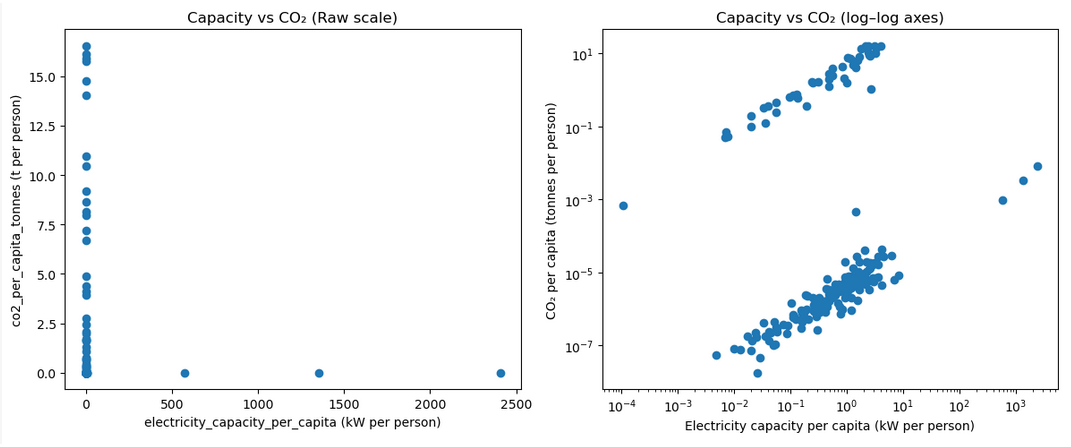
\includegraphics[width=1\linewidth]{pictures/rawVSlog.png}
    \caption{raw scale vs log-log scale example}
    \label{fig:rawvslog}
\end{figure}




\section{Task Analysis (Why)}\label{sec:taskAnalysis}

% his section focuses on tasks and is split into two subsections

\subsection{Domain Specific Tasks}
% in this section, you must analyze the possible visualization tasks
% that the users would be interested in doing, and you will solve them with your
% visualization design/tool. There might be tasks, especially low-level, that are not better
% solved with visualization, but combined with other tasks the overall becomes a
% visualization task or goal. Ideally, you present a set of tasks and corresponding
% questions that are related to the chosen domain and overall goal, which should be clear
% in the text. Notice that questions and tasks are similar in concept. Questions are often
% a useful way to clarify tasks. Present multiple tasks and also at different levels as
% presented in class. Some of the tasks should have a considerable level of complexity,
% e.g., involve multiple attributes where complex relations beyond a few (2 or 3)
% attributes need to be made. Notice that tasks do not refer to how the tool should look
% like but why the users should be using the visualization tool, independently of how it
% is visualized.


Given that our main goal is to help potential investors looking to find a suitable location to build data centers. It follows based on the studies on how investors should decide on factors for building data centers, involved profitability, interconnectedness, and sustainability. Note that this is not an exhaustive list, just the factors we will be investigating in the scope of this course. \\

%original task table -------------------- >:
\mycomment{
\textbf{T1 Accessibility: What countries are accessible and interconnected for maintenance and transfer of resources from the data center?}
\begin{itemize}
\item T1.1\quad Compare transportation infrastructure (road, rail, and airport density) across candidate countries to assess logistics capability. 
\item T1.2\quad Filter countries by water accessibility and availability to identify viable cooling possibilities.
\item T1.3\quad Characterize the distribution of broadband penetration and internet users to identify high-connectivity countries.
\end{itemize}

\textbf{T2 Profitability: Which countries are rich in capital and talent for running and maintaining the data centers?}
\begin{itemize}
\item T2.1\quad Rank GDP (and its trends) across candidate countries to assess economic potential.
\item T2.2\quad Characterize and compare the distribution of unemployment rate, literacy rate, and population growth to find countries with high workforce availability.
\end{itemize}

\textbf{T3 Efficiency: What are the most energy efficient and sustainable countries for building a data center for long term? }
\begin{itemize}
\item T3.1\quad Approximate which countries have relatively green energy systems, by low $CO_2$ emissions per unit of economic output and a lower share of fossil fuels in their energy mix.
\item T3.2\quad Find which countries provide the most reliable and efficient power supply for data centers, balancing electricity access, generation capacity, and emissions. (showing trade-offs)
\end{itemize}
}

\textbf{T1 Accessibility: What countries are accessible and interconnected for maintenance and transfer of resources from the data center?}
\begin{itemize}
\item T1.1\quad Analyze how transportation infrastructure varies across countries to understand logistical accessibility for data centers.
\item T1.2\quad Explore geographic and climatic conditions that influence cooling suitability, such as water availability and coastline exposure.
\item T1.3\quad Characterize global patterns in digital connectivity to identify countries with strong communication networks.
\end{itemize}

\textbf{T2 Profitability: Identify countries with strong economic conditions and human capital to maximize long-term returns from data center investments.}
\begin{itemize}
\item T2.1\quad Compare GDP per capita and real GDP growth rate across countries to identify economies with strong current performance and positive growth outlook.
\item T2.2\quad Discover countries with favorable labor markets by examining the distribution of youth unemployment rate, median age, and literacy rate across all countries.
\end{itemize}

\textbf{T3 Sustainability: Assess how sustainable the energy systems of different countries are for operating data centers at scale.}
\begin{itemize}
\item T3.1\quad Identify countries whose energy systems combine low carbon intensity with low fossil fuel dependence, indicating a higher potential for sustainable data center operation.
\item T3.2\quad Evaluate trade-offs between electricity access, generation capacity per capita, and emissions intensity to identify countries with reliable yet sustainable power supply.
\end{itemize}

\subsection{Task Abstraction}

\mycomment{
\begin{table}[h]
\centering
\setlength{\tabcolsep}{2pt} 
\begin{tabular}{p{0.04\textwidth} p{0.15\textwidth} p{0.26\textwidth}}
\textbf{Task} & \textbf{Action, Target} & \textbf{Justification} \\
\hline

T1.1 & Analyze / Compare (Many: Dependency) &
We use \textit{Analyze}, because the user’s goal is to understand how different independent infrastructure components (road, rail, airports) jointly affect accessibility. \\[0.2em]

T1.2 & Explore / Attributes (Many: dependency) &
Cooling suitability is not a single metric but emerges from combined effects of temperature, water share, and coastline, so users need to \textit{Explore} different combinations and thresholds interactively. \\[0.2em]

T1.3 & Characterize / Attributes (One/few: distribution) &
The goal for the user is to get an overview of connectivity levels worldwide, so \textit{Characterize} makes it so the user is understanding the distribution rather than inspecting individual cases. \\[0.4em]

T2.1 & Assess / Attributes (One/few: trends \& ranking) &
Investors want to \textit{Assess} which economies are more attractive by ranking and comparing GDP levels and growth, so that makes ordering and trend inspection key. \\[0.2em]

T2.2 & Analyze / Attributes (Many: distribution) &
\textit{Analyze} Unemployment rate, literacy rate, and population growth distributed across countries; so the user can find locations with strong workforce availability. \\[0.4em]

T3.1 & Analyze / Attributes (Many: composition + efficiency) &
To understand “greenness,” users must \textit{Analyze} both emissions intensity and fossil dependence together, not alone. \\[0.2em]

T3.2 & Explore / Attributes (Many: Dependency) &
There is no single best country; instead, users need to \textit{Explore} trade-offs between electricity access, capacity, and emissions to match their preferences. \\
\end{tabular}
\end{table}
}


% --- First half of the table ---
\begin{table}[H]
\centering
\setlength{\tabcolsep}{2pt} 
\caption{Task abstraction}
\begin{tabular}{p{0.04\textwidth} p{0.15\textwidth} p{0.26\textwidth}}
\textbf{Task} & \textbf{Action, Target} & \textbf{Justification} \\
\hline

T1.1 & Discover, (Many: Dependency) &
We use discover, because the user’s goal is to find new knowledge about different independent infrastructure components (road, rail, airports) jointly affect accessibility. \\[0.2em]

T1.2 & Explore, (Many: dependency) &
Users explore the visual space to find countries where climatic and geographic attributes (temperature, coastline, water resources) form favorable combinations for cooling. \\[0.2em]

T1.3 & Summarize, Attributes (One/few: distribution) &
Users summarize the distribution of connectivity indicators across all countries to understand the global pattern of strong vs. weak communication networks. \\[0.4em]

\end{tabular}
\end{table}

% --- Second half of the table (continued) ---
\begin{table}[H]
\ContinuedFloat
\centering
\setlength{\tabcolsep}{2pt} 
\caption[]{Task abstraction (continued)}
\begin{tabular}{p{0.04\textwidth} p{0.15\textwidth} p{0.26\textwidth}}

T2.1 & Compare, All data (One/few: trends) &
Users compare GDP level and growth trends between candidate countries to look for most attractive long‑term investment. \\[0.2em]

T2.2 & Discover, Attributes (Many: distribution) &
Users discover which countries offer strong workforce availability by examining the joint distribution of demographic and labour indicators across all countries \\[0.4em]

T3.1 & Identify, Attributes (Many: Dependency) &
Users identify which countries have greener energy systems by analysing dependencies between energy‑mix composition (fossil vs renewable) and emissions intensity. \\[0.2em]

T3.2 & Explore/Evaluate, Attributes (Many: Dependency) &
Users explore how electricity access, generation capacity, emissions intensity, and population size interact, identifying countries whose energy systems remain reliable and sustainable even when serving large populations. \\

\end{tabular}
\end{table}

\medskip

% Why: once you have defined a set of domain specific tasks, you must
% generalize them to be domain independent to be able to use the principles from
% visualization for the visual and interaction design. The tasks once abstracted do not
% contain domain language anymore but general data analysis visualization description

\section{Current Visualization and Interaction Design (How)}

% (How –you can give a name to your tool and use it as a section
% heading): In the interim report this is in development so it is not expected that this
% section is completely finished. Describe the current status of your visualization design,
% different elements, and components, and justify them. A Mock-up made on paper or a
% drawing tool is a good way to present your design. Also, add the justification to the
% level of possible at this point, i.e., justification from a perceptual point of view, and
% how your choices are related to design principles into account for the choice of marks
% and channels. How it fits the abstract tasks and data described in previous sections.
% You can also describe alternatives that you discarded and indicate why. If needed,
% provide some support by citing relevant literature. This section should NOT be a
% manual of your tool, but an explanation and justification of your design and what
% makes it possible. Whether you click the right button of the mouse or something else
% is not important for this project, but you are able to take the action is what matters.

% \subsection{Interaction Design}
The current dashboard integrates a map with filter options, a bar chart, a parallel coordinates plot, a scatter plot, and a spider plot. Each is selected to support the abstracted tasks defined in the earlier sections. The dashboard can be viewed in both light and dark mode to allow users to experience the benefits of both modes and use it according to their preferences. The marks and channels used are from Munzner's rank of marks and channels in order \cite{munzner2014visualization}
\smallskip



\noindent\textbf{Choropleth map and filtering overview.}\\
The dashboard begins with a map that gives an overview of all countries \autoref{fig:choropleth}. Filters can be applied to filter countries that fall in the range of the selected metric. The countries that satisfy the filters are highlighted in green while the others are blacked out, using a single hue to maximize the data‑ink ratio and keep the map visually simple. Within the selected set, we vary the lightness of the green to encode the actual metric value, leveraging the eye’s high sensitivity to changes in luminance around greenish wavelengths for better discriminability of magnitude differences\cite{GigahertzOptikEyeSensitivity}. While luminance is ranked 6th among Munzner’s effectiveness ordering, it gives our users an intuitive and clear overview of which countries satisfy tasks as T1.3, T2.1, T3.2. We use color hue to differentiate between countries that satisfy the filters and the countries that do not since color hue is the most effective identity channel for categorical attributes \cite{munzner2014visualization}.\\\\
Choropleth maps have the issue that large countries are more prominent than others. This could result in users overseeing small countries that would actually be interesting for the them. To help and solve this problem the bar chart can be used. The bar chart displays the 10 best countries displayed of the same metric that is encoded in the choropleth map. So, even if the user only noticed the larger countries in the map, they will be able to see the smaller countries in an equal way in the bar chart under it.

\begin{figure}[h!]
    \centering
    \includegraphics[width=1\linewidth]{pictures/worldMap.jpeg}
    \caption{Choropleth map with Luminance as the color channel}
    \label{fig:choropleth}
\end{figure}

\noindent\textbf{Bar chart} \\
For tasks that involve ranking and/or comparing countries based on a specific metric (such as T1.1, T1.3, T2.1), we use a bar chart \autoref{fig:barchart}. For marks, we use lines so that we can exploit two of the most effective magnitude channels for ordered attributes: length and position on a common scale. As the task is to rank the countries, the bars are sorted by the plotted value to support quick identification of extremes. All non-selected bars share the same neutral gray color, with only the highlighted bar differing; this reduces non-essential variation and follows Tufte’s data–ink principle by devoting most ink to the data values rather than decorative encoding differences.\\


\begin{figure}[h!]
    \centering
    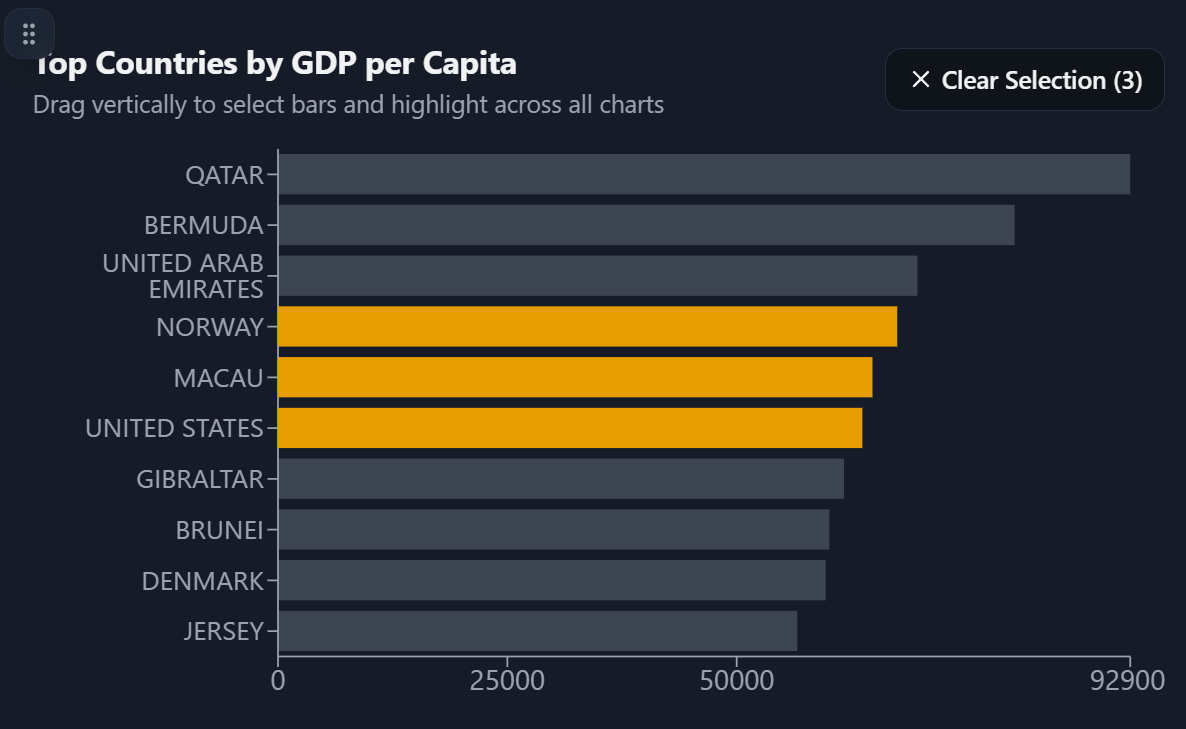
\includegraphics[width=1\linewidth]{pictures/barChart.png}
    \caption{Bar chart}
    \label{fig:barchart}
\end{figure}

\noindent\textbf{Parallel coordinates plot}\\
Some tasks (such as T1.1, T1.2, T1.3, T2.2, T3.1) require comparison of multiple interrelated attributes per country. The parallel coordinates plot supports this by allowing the user to trace a country across several axes and compare its profile both within and between countries \autoref{fig:pcp}. Its primary encoding is position on a common scale for each attribute, which is well suited for comparing ordered values across many dimensions. Initially, all poly lines share the same neutral gray, so almost all ink is devoted to representing data rather than decorative styling, in line with Tufte’s data–ink principle; when a country is selected in any view, its line is highlighted in a distinct hue so that it can be followed easily across axes without introducing unnecessary color variation. The user can configure which attributes appear as axes, and both quantitative and categorical variables can be included, enabling flexible multivariate comparisons within a single coordinated view. \\

\begin{figure}[h!]
    \centering
    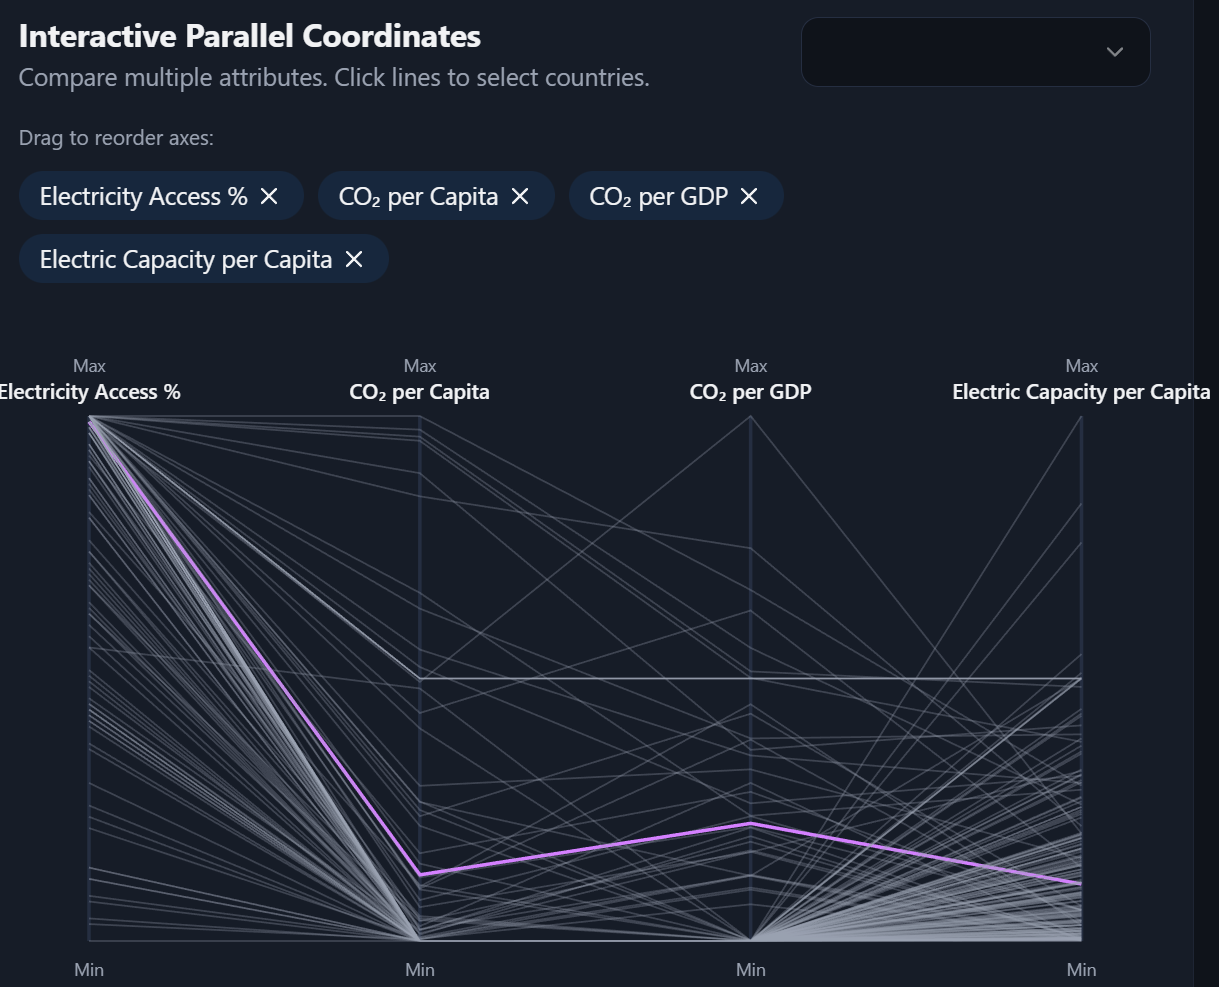
\includegraphics[width=0.98\linewidth]{pictures/parallelcordplot.png}
    \caption{Parallel coordinates plot}
    \label{fig:pcp}
\end{figure}

\noindent\textbf{Scatter plot}\\
The scatterplot \autoref{fig:scatter} supports in-depth identification of relationships between quantitative variables for tasks T1.3, T2.2, T3.1, and T3.2. Positions on common scales encode the two main attributes, leveraging the most accurate magnitude channel for ordered data. A third quantitative attribute is currently encoded through bubble size; while this allows users to notice large differences in magnitude, area is a relatively low-precision channel and large bubbles may occlude smaller ones, making it harder to judge fine-grained differences or see dense regions clearly. In the final report, this design could be extended into a scatterplot matrix (SPLOM), replacing bubble size with multiple 2D plots so that higher-dimensional correlations can be inspected using position alone, which provides more reliable comparisons across many attribute pairs\cite{munzner2014visualization}.


\begin{figure}[h!]
    \centering
    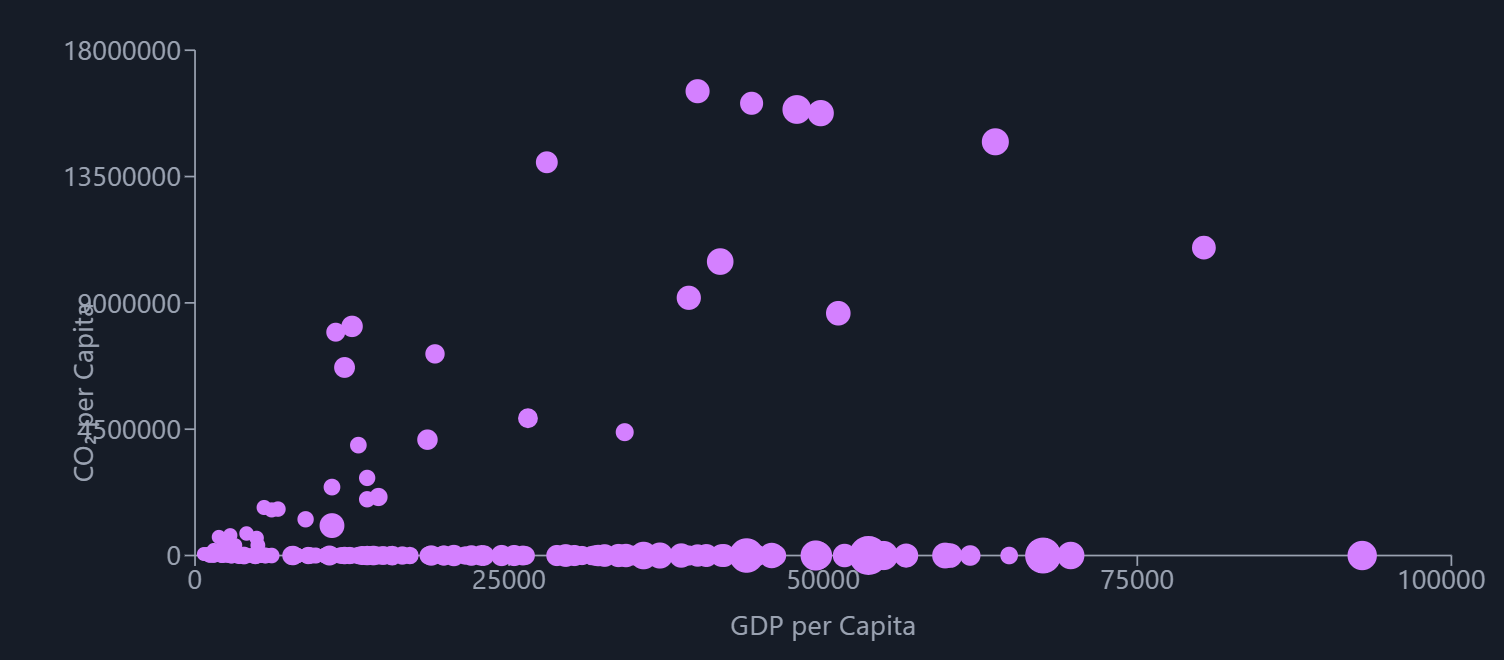
\includegraphics[width=0.98\linewidth]{scatterplot.png}
    \caption{Scatterplot}
    \label{fig:scatter}
\end{figure}

\noindent\textbf{Spider plot}\\
When a country is selected somewhere, this country will be shown in the spider plot. Here \autoref{fig:spider}, the user can see the scores of this country across the seven most significant metrics. In this way, the user can see at a glance if this country is actually what they are looking for and even compare between candidate countries. The spider plot thus mostly accommodates the higher level tasks where the user wants to compare a smaller subset of countries to determine which one is more suitable in what area.

As mentioned in Section 2, some countries/territories have been entirely deleted from the dataset due to missing core data and some were not even countries bu. Even though those countries were deleted some countries might still have missing values. But these are considered non vital for the user to make a decision. However, to maintain graphical integrity, we report the missing values in the plot instead of deleting the country or setting the value to zero. \\

\begin{figure}[h!]
    \centering
    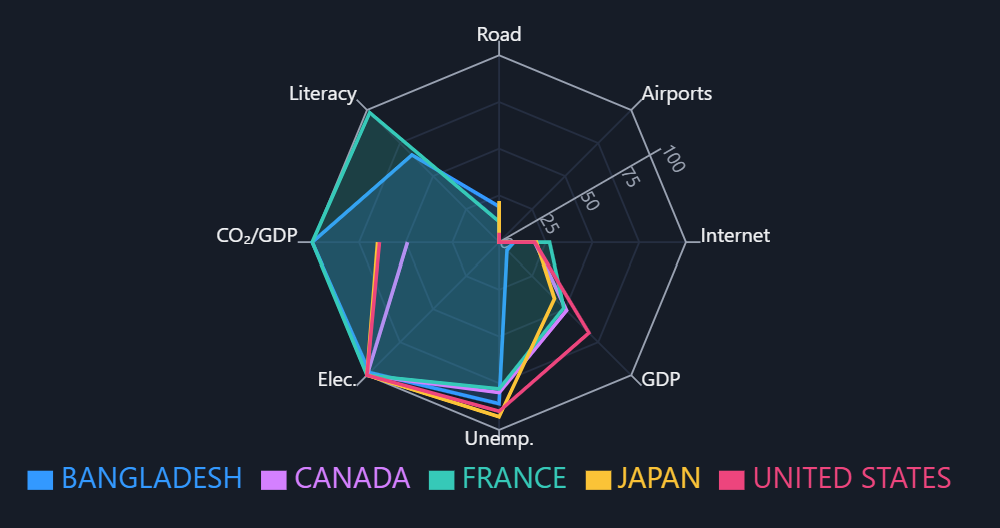
\includegraphics[width=0.95\linewidth]{pictures/spiderplot.png}
    \caption{The plot shows with missing data for literacy as talked about earlier, it's set to Null and it's still showing comparing relative to others and not connecting for missing values such as \textit{literacy rate}}
    \label{fig:spider}
\end{figure}


\noindent\textbf{Interaction across visualizations} \\
The visualizations are tightly linked: selecting a country in any view highlights the corresponding item across all other views. All plots are bidirectionally connected to the map, so clicking a country on the choropleth highlights the corresponding bar in the bar chart, the poly line in the parallel coordinates plot, and the segment in the spider plot. This coordinated highlighting leverages the Gestalt principle of similarity and common fate: using the same color and simultaneous motion (appearance/disappearance of highlights) helps users immediately perceive these marks as belonging to the same country across multiple representations.

\smallskip
\begin{figure}[h!]
    \centering
    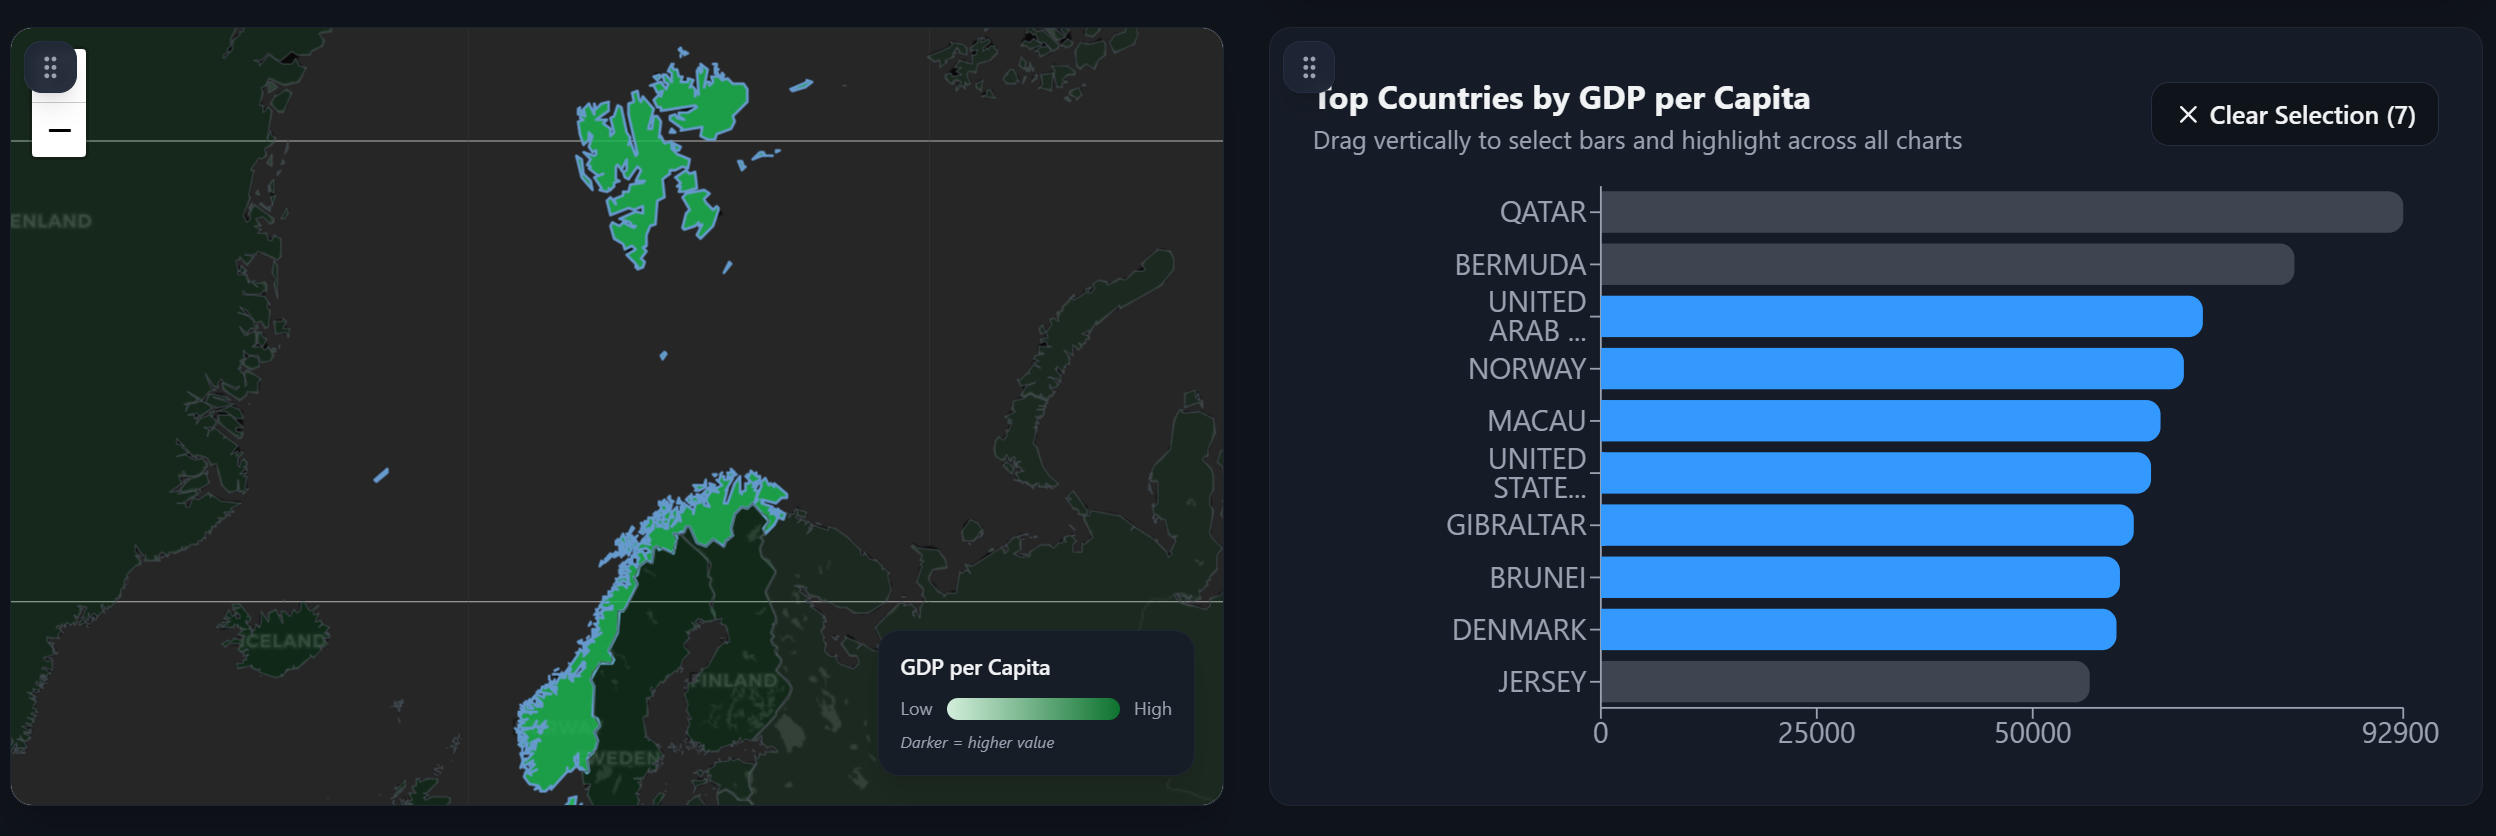
\includegraphics[width=0.95\linewidth]{pictures/linking_brushing.png}
    \caption{Brushing and linking between the choropleth map and the GDP-per-capita bar chart, where selecting countries in one view highlights the corresponding items in the other.}
    \label{fig:linkingandbrushing}
\end{figure}

\noindent To reduce reliance on memory, the dashboard layout is flexible: users can drag and place the plots next to the map to compare values side by side instead of scrolling, so that “eye beats memory.” As illustrated in Figure~\ref{fig:linkingandbrushing}, brushing and linking between the map and bar chart ensures that selecting countries in one view immediately reveals their counterparts in the other, supporting rapid comparison without mentally tracking identifiers across views.



\section{Aggregation and Interaction Design}
This section extends the current visualization design by introducing clustered exploration, richer coordination between views, and dimensionality reduction to better support the abstracted tasks in Section~\ref{sec:taskAnalysis}.

\subsection{Aggregation via Clustering for T1.1}
For task T1.1 (analyzing how transportation infrastructure varies across countries), aggregating individual countries into \textbf{clusters} helps users see broader logistical patterns that are obscured when showing all 199 countries separately. Instead of inspecting single countries, users can compare groups with similar infrastructure profiles, which better supports high-level investment screening and avoids overplotting in both the choropleth and multivariate views~\cite{elmqvist2010hierarchical}.

To construct these groups, the dashboard applies k-means clustering on standardized infrastructure attributes: \textit{road\_density\_per\_1000km2}, \textit{rail\_density\_per\_1000km2}, \textit{airports\_per\_million}, and optionally \textit{internet\_users\_per\_100} to provide connectivity context. The number of clusters $k$ is determined using the elbow method or silhouette analysis to balance interpretability with separation quality. The resulting cluster labels are then:

\begin{itemize}
    \item Encoded on the \textbf{SPLOM} (scatterplot matrix) using color hue, allowing users to visually inspect separation and overlap between clusters across multiple attribute pairs. This leverages hue as the most effective identity channel for categorical data~\cite{munzner2014visualization}.
    \item Mapped onto the \textbf{choropleth}, where each country is colored by its cluster membership while luminance continues to indicate the magnitude of the currently selected metric, preserving comparability with the existing design.
\end{itemize}

This combination allows users to quickly identify, for example, clusters of countries with dense road and air networks but weaker rail infrastructure, and then inspect how these groups distribute geographically---directly supporting the ``Discover'' action abstracted in T1.1.

\subsection{Dimensionality Reduction via PCA}
Some thematic groups---such as energy systems, macroeconomic indicators, or environmental risk factors---contain many correlated attributes (around 25 in total), which can overload both parallel coordinates and scatterplots. To address this, the dashboard incorporates \textbf{Principal Component Analysis (PCA)} as a preprocessing step, projecting each high-dimensional attribute block into a small number of orthogonal components while retaining most of the variance~\cite{jolliffe2016pca}.

These principal components are:
\begin{itemize}
    \item Exposed as additional axes in the parallel coordinates plot (e.g., ``Energy PC1: low-carbon vs fossil-heavy'', ``Infrastructure PC1: high vs low density''), making it easier to compare countries along interpretable composite directions.
    \item Used as dimensions in the SPLOM, reducing clutter and helping users detect global patterns (e.g., countries that are simultaneously strong on infrastructure and green energy) using only position encoding.
\end{itemize}

A potential concern is that principal components lose interpretability compared to raw attributes. To mitigate this, the dashboard displays component loadings on demand via tooltip, so users can understand which original attributes contribute most to each component. This preserves transparency while reducing visual complexity.

\subsection{Interaction Idioms for Analytical Tasks}
The dashboard supports several of Munzner's interaction categories through coordinated multiple views that link the choropleth map, bar chart, parallel coordinates, scatterplots/SPLOM, and spider plot~\cite{roberts2007state}:

\begin{itemize}
    \item \textbf{Select}: Clicking a country on the choropleth selects it and highlights the corresponding bar, polyline, point, and polygon across all views, using a shared color to leverage the Gestalt principle of similarity.
    \item \textbf{Explore}: Users explore relationships between attributes by scanning the parallel coordinates axes and scatterplots; extending to a SPLOM enables systematic inspection of bivariate relationships across all infrastructure and energy attributes using position as the primary magnitude channel.
    \item \textbf{Reconfigure}: The layout is draggable, so users can place views side by side, reducing reliance on memory (``eye beats memory''~\cite{munzner2014visualization}). A planned extension allows reordering axes in the parallel coordinates plot to reveal correlations between adjacent dimensions.
    \item \textbf{Encode}: Currently, the map uses a single hue with varying luminance to encode the selected metric. Future work could allow users to switch color schemes (e.g., perceptually uniform sequential scales from ColorBrewer~\cite{brewer2003colorbrewer}) or toggle log/linear scale on axes.
    \item \textbf{Abstract/Elaborate}: Hovering on a country reveals details-on-demand, including raw values and z-scores, helping users move seamlessly between high-level patterns and precise numeric information.
    \item \textbf{Filter}: Range sliders connected to the map and bar chart let users restrict the view to countries within a specified range; a natural extension is multi-attribute filtering (e.g., ``road density $>$ X AND renewable share $>$ Y''), which would immediately propagate to all linked views.
    \item \textbf{Connect}: Brushing and linking are implemented bidirectionally: selections in any view propagate to all others, so users can trace the same country or cluster across all visualizations without mentally matching labels.
\end{itemize}

\subsection{Data Center Overlay for Validation}
An external dataset of existing data-center locations (\textit{datacenter\_location.csv}, containing 193 countries with attributes such as total data centers, hyperscale count, and power capacity) can be overlaid as an additional categorical or quantitative layer on the choropleth. This supports a compare-and-contrast task: users can see where data centers already exist and evaluate whether candidate countries with favorable infrastructure scores but few existing facilities represent untapped opportunities or have hidden barriers. This directly addresses the domain goal of site selection by grounding the analysis in real-world deployment patterns.

Together, clustering, PCA, and enhanced interaction idioms provide higher-level abstractions that still remain grounded in the original metrics, thereby supporting both overview-first exploration and detailed comparison within the same coordinated, interactive environment.

\section{Implementation}
We used Pandas and Numpy in Python to pre-process the raw CSV files from Kaggle's CIA World Factbook datasets that underpin our AI data center location dashboard.
\smallskip
The interactive dashboard is implemented as a web application using React, Typescript, and Tailwind CSS. Geo-spatial visualization is handled with Leaflet via the React-Leaflet bindings. The deployed dashboard is available at
\href{https://visgroup13.vercel.app/}{\texttt{visgroup13.vercel.app}}
alongside the source code on
\href{https://github.com/MuhammadIbneRafiq/visualization-13}{\texttt{github.com/MuhammadIbneRafiq/visualization-13}}. Please note that some of the features may still contain bugs as it's still a work in progress.

\bibliographystyle{abbrv}
% \bibliographystyle{abbrv-doi}
% \bibliographystyle{abbrv-doi-narrow}
% \bibliographystyle{abbrv-doi-hyperref}
%\bibliographystyle{abbrv-doi-hyperref-narrow}
% \bibliographystyle{IEEEtran}


\bibliography{template}
\end{document}
